\documentclass[12pt, a4paper,twoside]{article}

\begin{document}
\label{sec:workDone}
	Estimating correspondences between images is one the fundamental problems in computer vision\cite{20AA} with applications ranging from large-scale 3D reconstruction to image manipulation and semantice segentation \cite{44AA}.In this project, My first challenge is to build on the traditional approach and develop a convolutional neural network (CNN) architecture that mimics the standard matching process and will replace the standard local features with powerful trainable convolutional neural network features \cite{33AA}, which allows us to handle large changes of appearance between the matched images. The outcome is a convolutional neural network architecture trainable for the end task of geometric matching,which can handle large appearance changes, and is therefore suitable for both instance-level and category-level matching problems. 

	My second task was to provide a matching layer at the end which can handle sensor inter-operability issues. In heterogeneous sensor environment, it is crucial to identify the source sensor by which the acquired image is captured. This is essentially required to handle sensor inter-operability issues and further in identifying various attacks on biometric systems, where biometric templates can be modified or mis-used. Another interesting application of sensor identification is in establishing the sequence of commands for law enforcement to identify spurious activities in online systems. An image can be altered or fabricated during the acquisition phase, transmission or during storage. In order to understand whether the image has been fabricated or not it is necessary to know the source that generates the image

	Fingerprint sensors can be classified into various categories e.g. (i) basis of imaging technology they are classified as optical, capacitive and thermal; (ii) basis of user interaction they are classified as press, sweep and non-contacted ones. Fig~\ref{fig:figure2} shows fingerprint images captured from different types of sensors. It is evident from Fig~\ref{fig:figure2}, that image quality largely depends upon underlying sensor employed.

\begin{figure}[htbp]
\centering
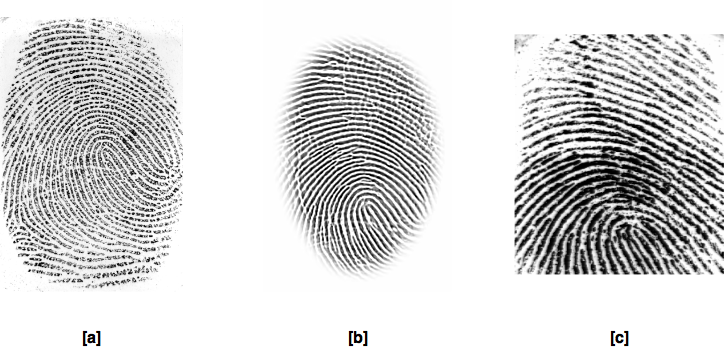
\includegraphics[scale=0.5]{images/differentSensorsOutputs}
\caption{Example of fingerprint images taken from different sensors (a) Futronic, (b) Lumidigm, (c) SecuGen
}\label{fig:figure2}
\end{figure}


\end{document}
 
 
